\section{Режимы работы блочных шифров}\label{section-block-chaining}
\selectlanguage{russian}

Перед шифрованием открытый текст $M$ разбивают на части $M_1, M_2, \dots, M_n$, называемые \emph{блоками шифрования}\index{блок!шифрования}. Размер блока зависит от используемого блочного шифра, и, как упоминалось ранее, для шифра <<Магма>>\index{шифр!Магма} он составляет 64 бита, для AES\index{шифр!AES} и шифра <<Кузнечик>>\index{шифр!Кузнечик} -- 128 бит.
    \[ M = M_1 || M_2 || \dots || M_i. \]

Размер открытого текста может быть не кратен размеру блока шифрования. В этом случае для последнего блока применяют процедуру дополнения (удлинения) до стандартного размера. Процедура должна быть обратимой: после расшифрования последнего блока пакета лишние байты необходимо обнаружить и удалить. Некоторые способы дополнения:
\begin{itemize}
  \item добавить один байт со значением $128$, а остальные байты принять за нулевые;
  \item определить, сколько байтов надо добавить к последнему блоку, например $b$, и добавить $b$ байтов со значением $b$ в каждом.
\end{itemize}

После шифрования всех блоков открытого текста (блоков шифрования) получается набор блоков шифртекста $C_1, C_2, C_3, \dots, C_n$. Обычно размер этих блоков равен размеру блока шифрования (точно не может быть меньше блока шифрования). Процедура, по которой этот из этого набора блоков получается итоговый шифртекст, называется режимом работы блочного шифра. Некоторые режимы работы могут оперировать не только блоками шифртекста, но и исходными блоками шифрования, номерами блоков и специальными векторами инициализации.

Существует несколько режимов работы блочных шифров: режим электронной кодовой книги, режим шифрования зацепленных блоков, режим обратной связи, режим шифрованной обратной связи, режим счётчика. Рассмотрим особенности каждого из этих режимов.

\subsection{Электронная кодовая книга}
\selectlanguage{russian}

\begin{figure}[bt]
	\centering
	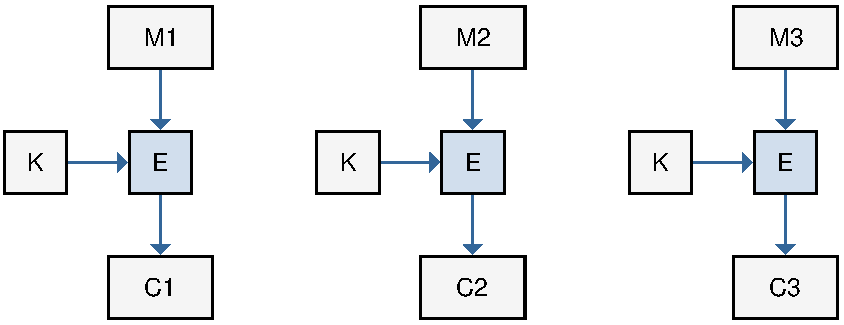
\includegraphics[width=1\textwidth]{pic/ECB}
	\caption{Режим электронной кодовой книги}
	\label{fig:ECB}
\end{figure}

В стандарте ГОСТ 28147-89 данный режим называется \emph{режимом простой замены}.~\cite{GOST-89}

В режиме электронной кодовой книги (\langen{Electronic Code Book, ECB}, рис.~\ref{fig:ECB}) открытый текст в пакете разделён на блоки
    \[ \left[ M_1, M_2, \dots, M_{n-1}, M_n \right]. \]

В процессе шифрования каждому блоку $M_j$ ставится в соответствие шифртекст $C_j$, определяемый с помощью ключа $K$:
    \[ C_j = E_K(M_j), ~ j = 1, 2, \dots, n. \]

Если в открытом тексте есть одинаковые блоки, то в шифрованном тексте им также соответствуют одинаковые блоки. Это даёт дополнительную информацию для криптоаналитика, что является недостатком этого режима. Другой недостаток состоит в том, что криптоаналитик может подслушивать, перехватывать, переставлять, воспроизводить ранее записанные блоки, нарушая конфиденциальность\index{конфиденциальность} и целостность\index{целостность} информации. Поэтому при работе в режиме электронной кодовой книги нужно вводить аутентификацию сообщений.

Шифрование в режиме электронной кодовой книги не использует сцепление блоков и синхропосылку\index{синхропосылка} (вектор инициализации)\index{вектор инициализации}. Поэтому для данного режима применима атака на различение сообщений, так как два одинаковых блока или два одинаковых открытых текста шифруются идентично.

На рис.~\ref{fig:ecb-demo} приведён пример шифрования графического файла морской звезды в формате BMP, 24 бита цветности на пиксель (рис.~\ref{fig:starfish}), блочным шифром AES с длиной ключа 128 бит в режиме электронной кодовой книги (рис.~\ref{fig:starfish-aes-128-ecb}). В начале зашифрованного файла был восстановлен стандартный заголовок формата BMP. Как видно, в зашифрованном файле изображение всё равно различимо.
\begin{figure}[!ht]
    \centering
    \subcaptionbox{Исходный рисунок\label{fig:starfish}}{ 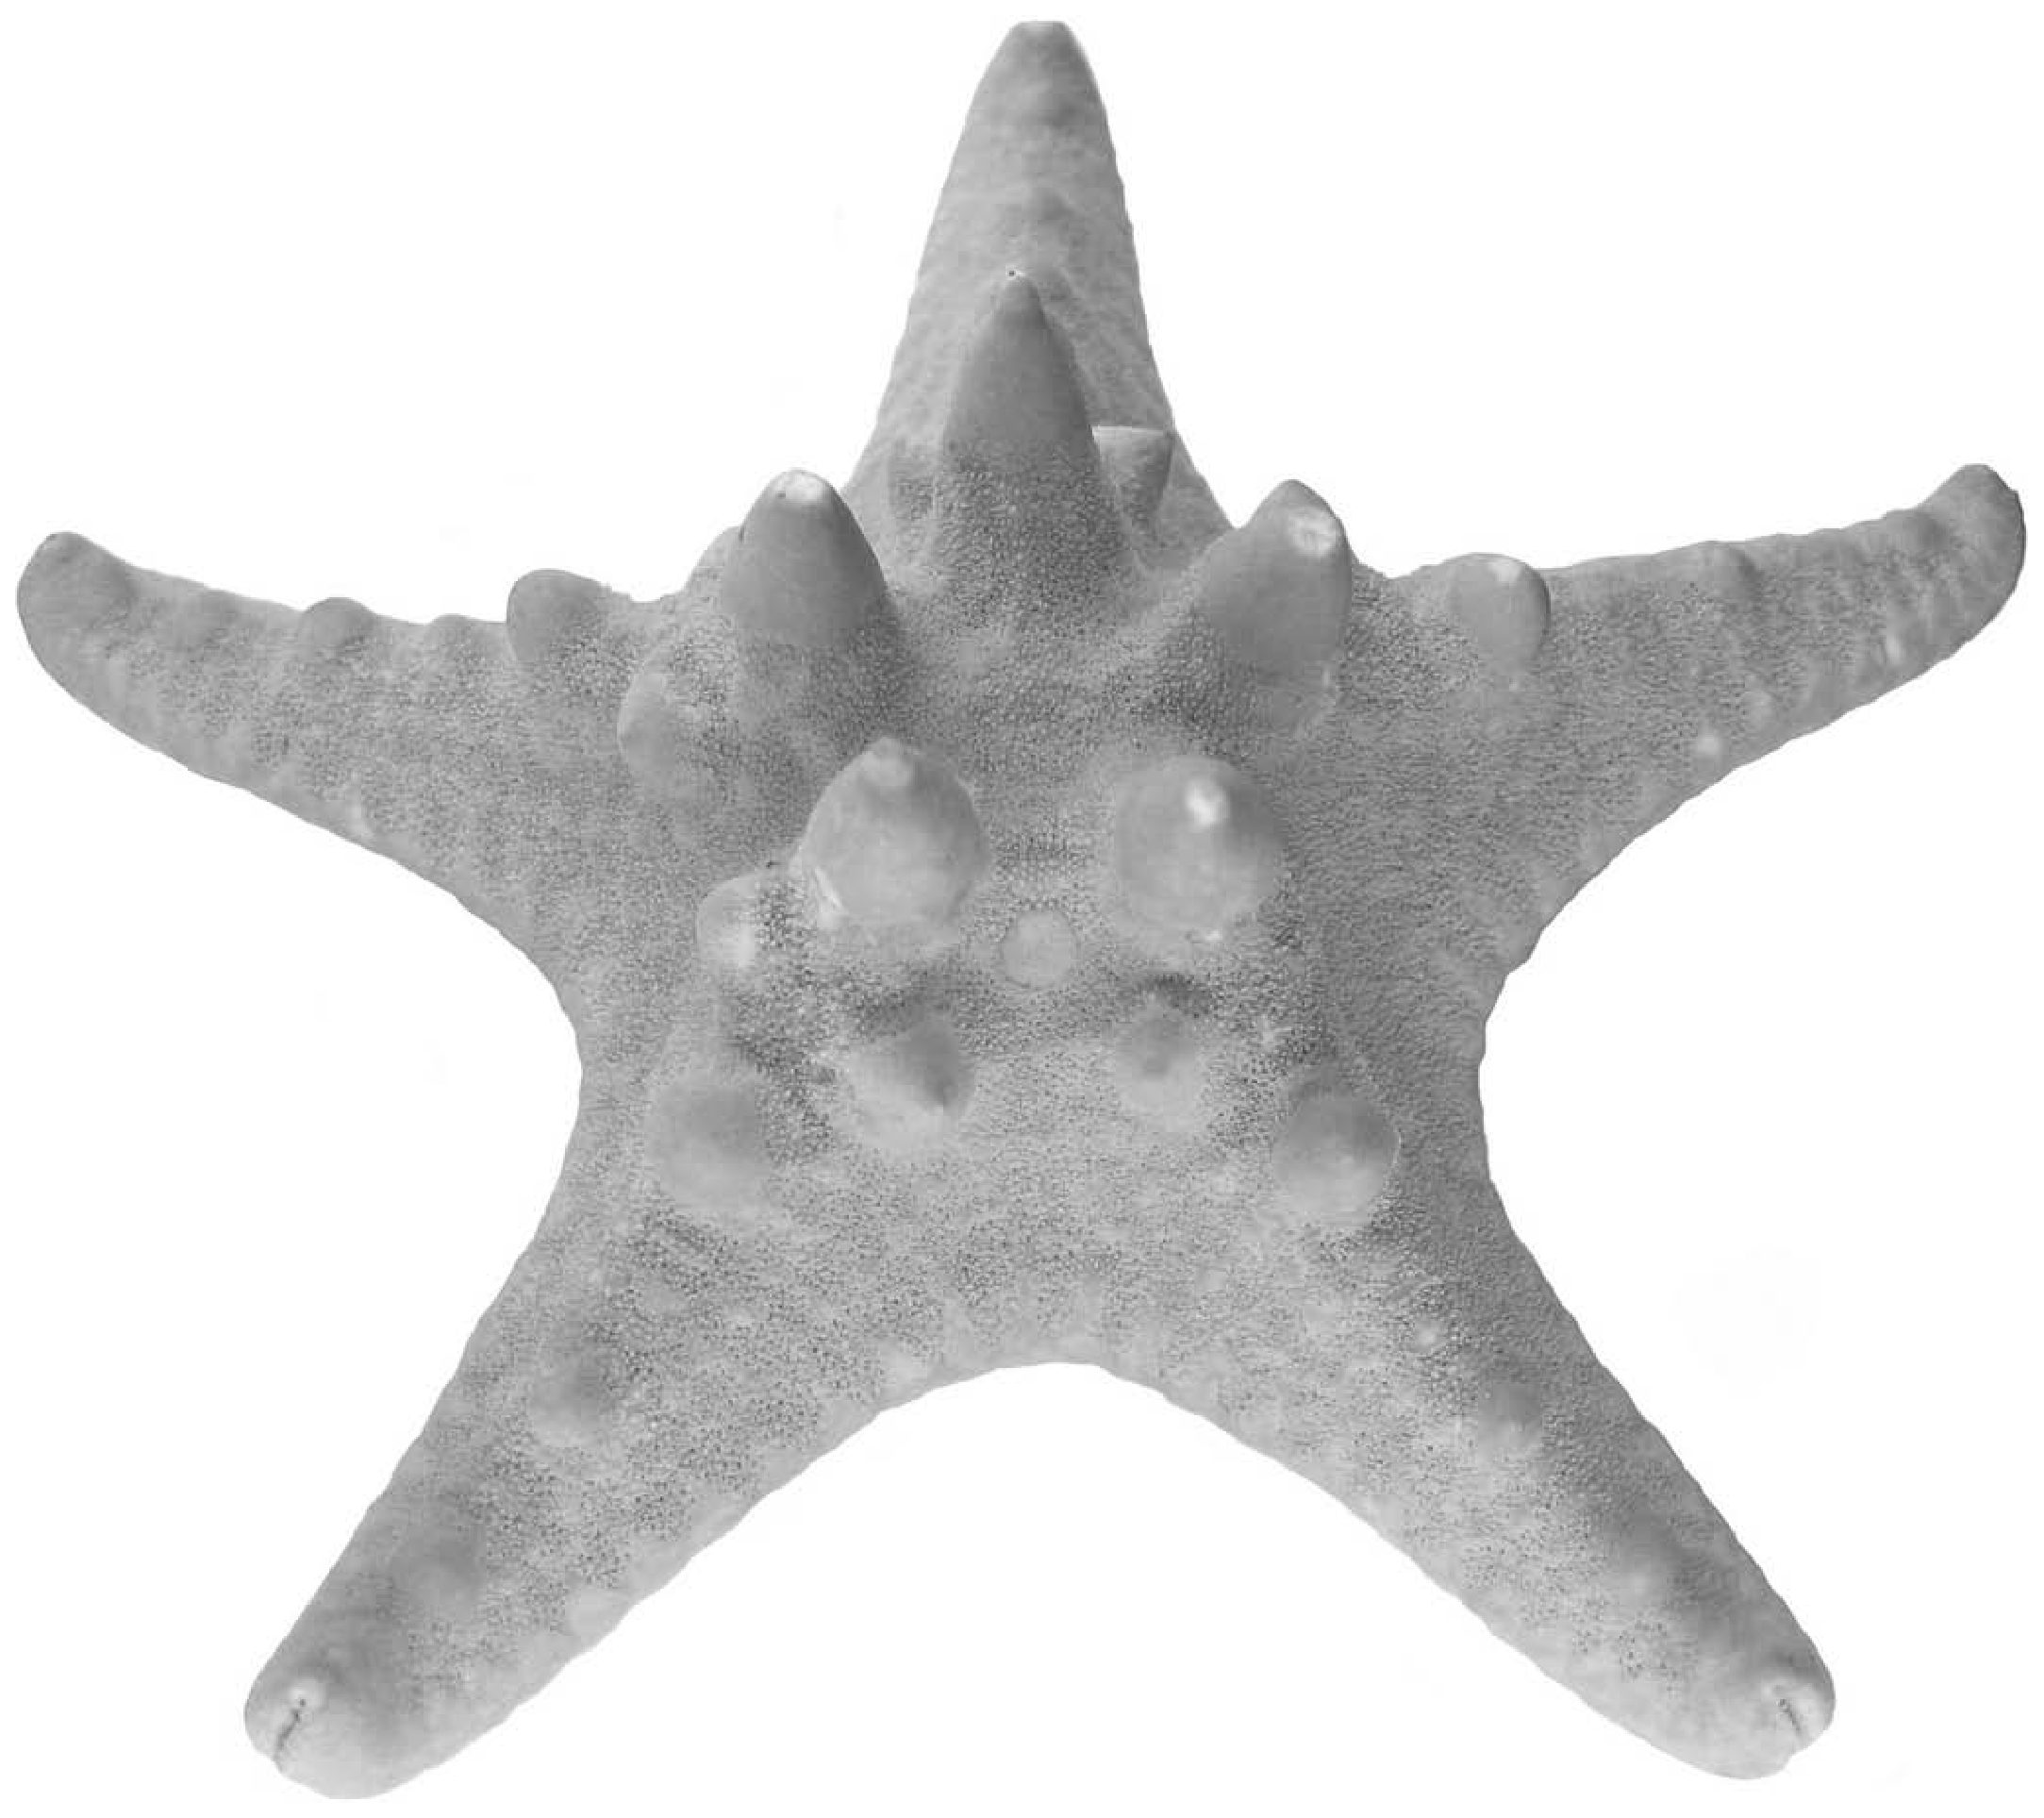
\includegraphics[width=0.45\textwidth]{pic/starfish}}
    ~~~
    \subcaptionbox{Рисунок, зашифрованный AES-128\label{fig:starfish-aes-128-ecb}}{ 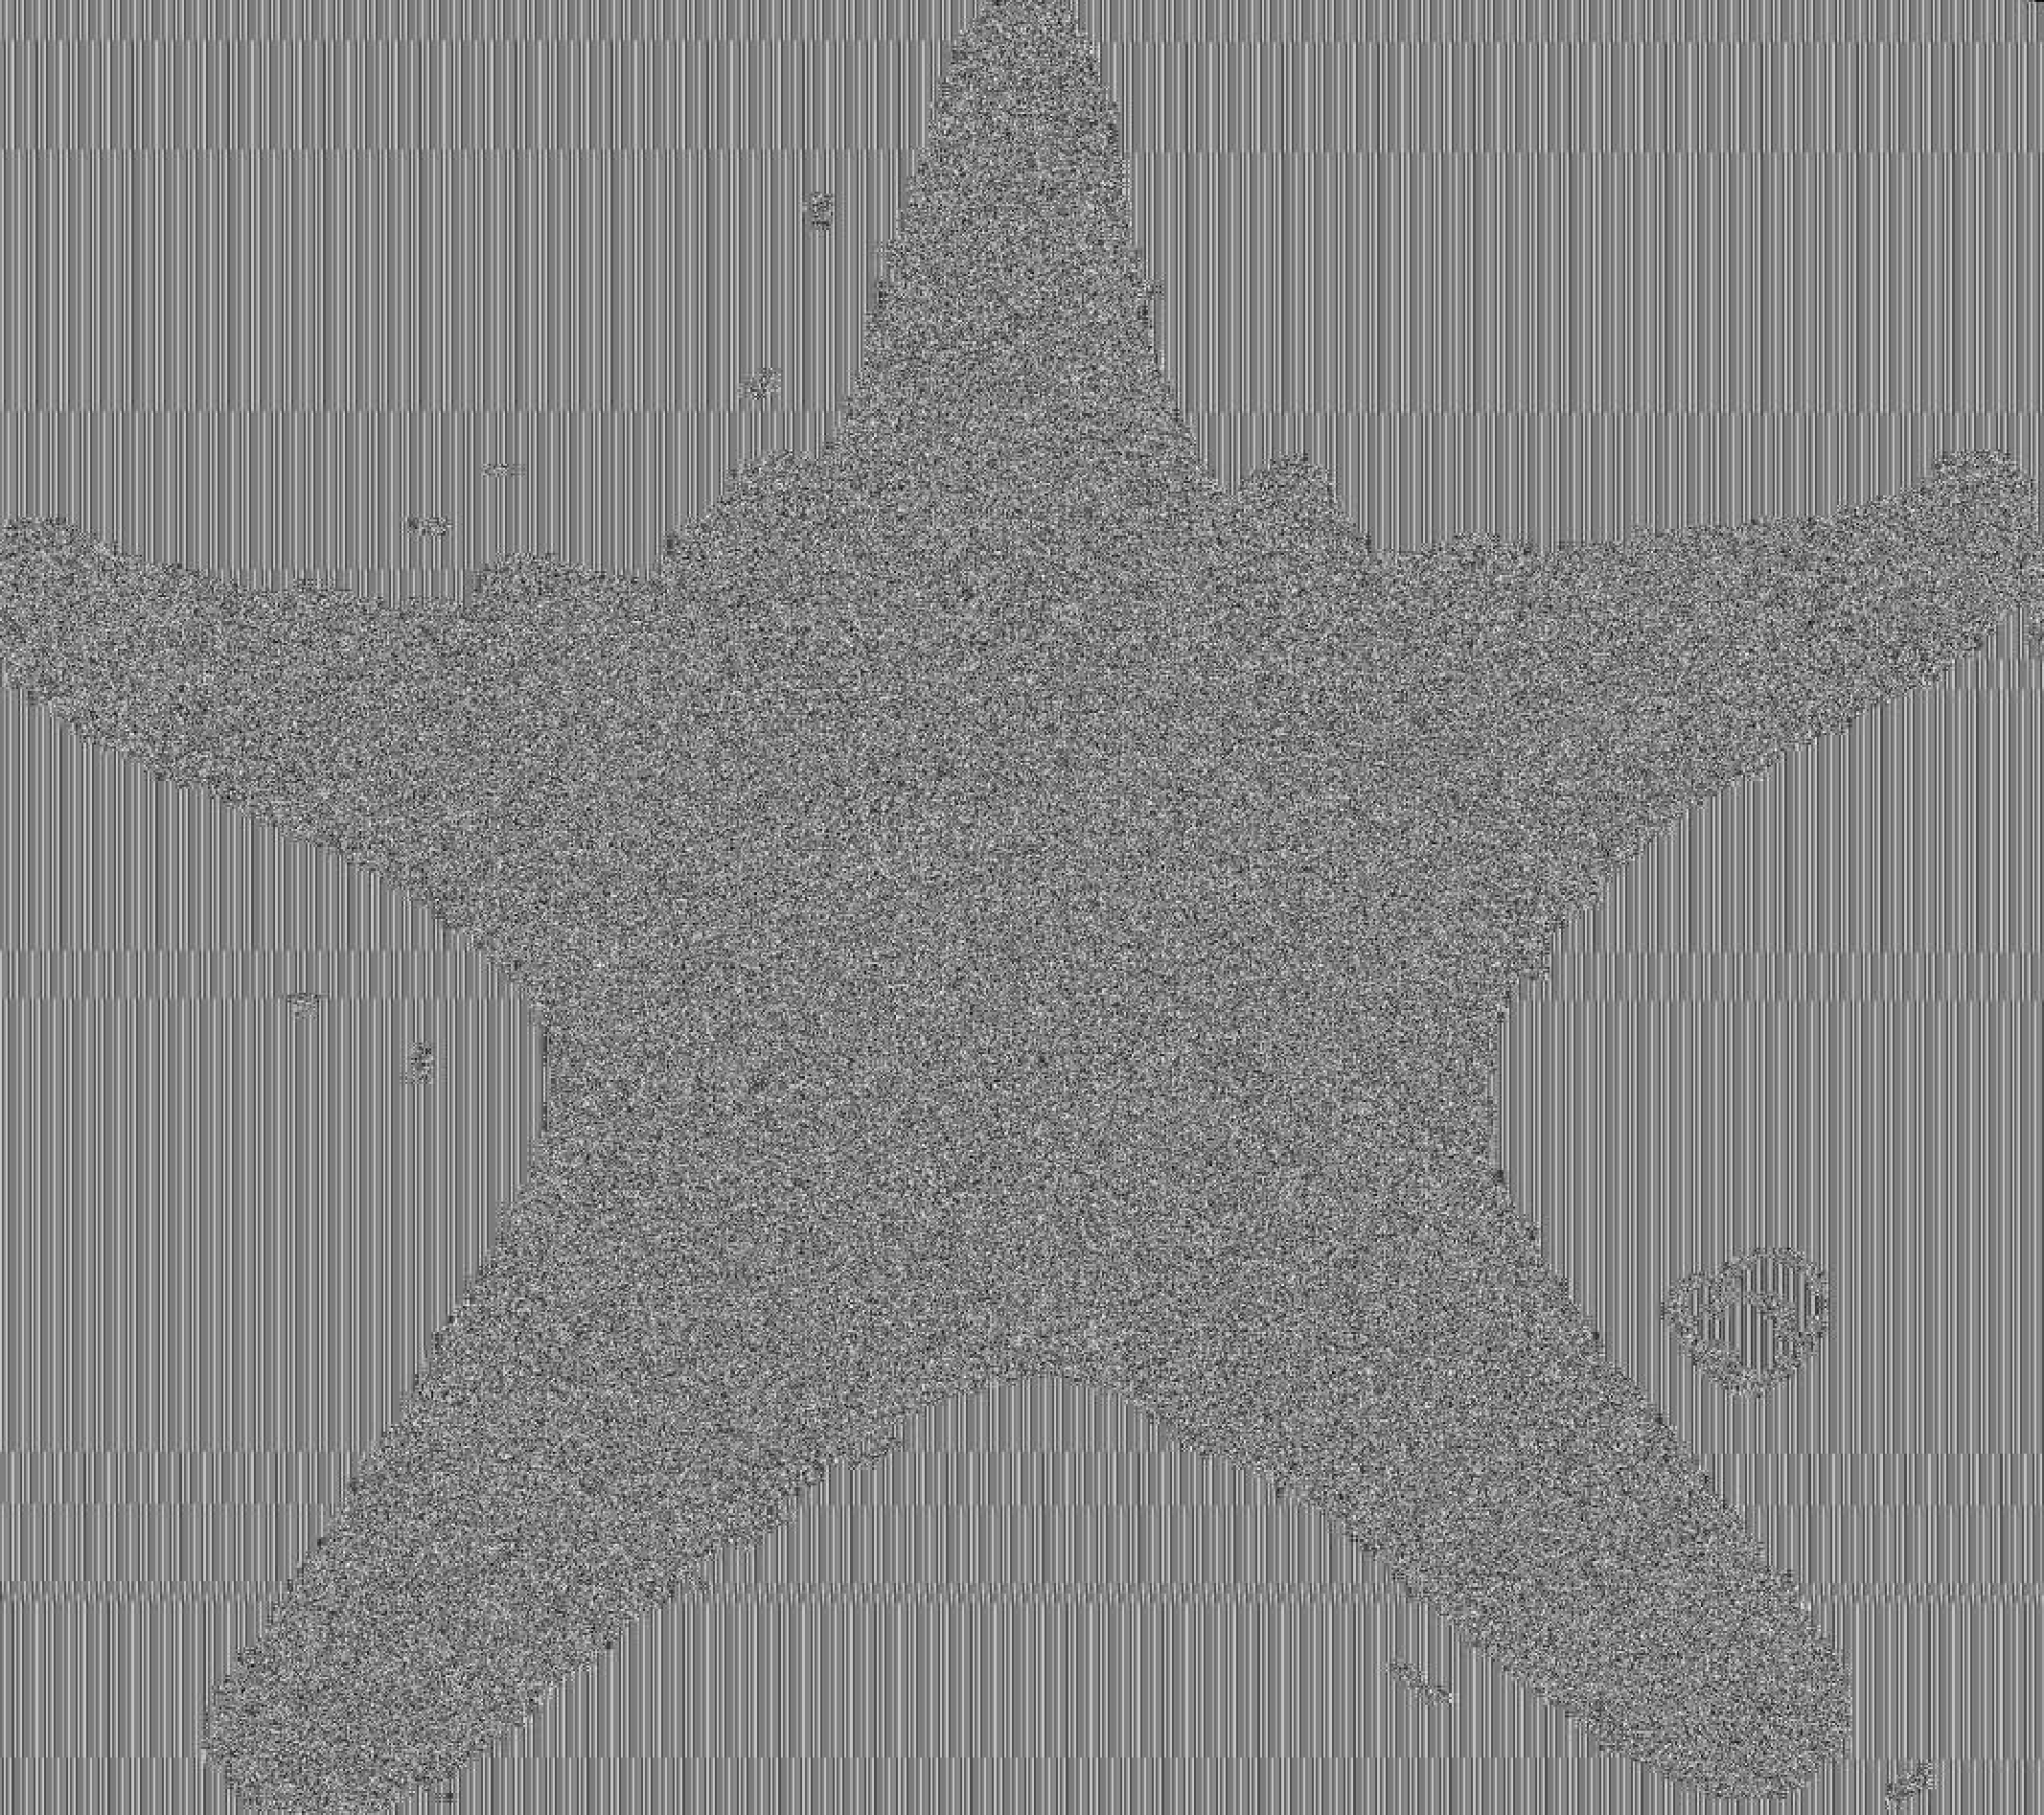
\includegraphics[width=0.45\textwidth]{pic/starfish-aes-128-ecb}}
    \caption{Шифрование в режиме электронной кодовой книги\label{fig:ecb-demo}}
\end{figure}
BMP файл в данном случае содержит в самом начале стандартный заголовок (ширина, высота, количество цветов), и далее идёт массив 24-битовых значений цвета пикселей, взятых построчно сверху вниз. В массиве много последовательностей нулевых байтов, так как пиксели белого фона кодируются 3 нулевыми байтами. В AES размер блока равен 16 байтам, и, значит, каждые $\frac{16}{3}$ подряд идущих пикселей белого фона шифруются одинаково, позволяя различить изображение в зашифрованном файле.

%На рис.~\ref{fig:ecb-demo} приведён пример шифрования графического файла логотипа Википедии в формате BMP, 24 бита цветности на пиксель (рис.~\ref{fig:wikilogo}), блочным шифром AES с длиной ключа 128 бит в режиме электронной кодовой книги (рис.~\ref{fig:wikilogo-aes-128-ecb}). В начале зашифрованного файла был восстановлен стандартный заголовок BMP формата. Как видно, на зашифрованном рисунке возможно даже прочитать надпись.
%\begin{figure}[!ht]
%    \centering
%    \subfloat[Исходный рисунок]{\label{fig:wikilogo}\includegraphics[width=0.45\textwidth]{pic/wikilogo}}
%    ~~~
%    \subfloat[Рисунок, зашифрованный AES-128]{\label{fig:wikilogo-aes-128-ecb}\includegraphics[width=0.45\textwidth]{pic/wikilogo-aes-128-ecb}}
%    \caption{Шифрование в режиме электронной кодовой книги.}
%    \label{fig:ecb-demo}
%\end{figure}

%Возможно воссоздание структуры информации -- например, пингвин на рис.~\ref{fig:tux-ecbmode}. Картинка с пингвином записана в формате BMP и зашифрована DES в режиме электронной кодовой книги.
%\begin{figure}[!ht]
%    \centering
%    \includegraphics[width=0.3\textwidth]{pic/tux-ecb}
%    \caption{Картинка с пингвином, зашифрованная в режиме электронной кодовой книги.}
%    \label{fig:tux-ecbmode}
%\end{figure}

К плюсам данного режима шифрования можно отнести:

\begin{itemize}
	\item возможность параллельного шифрования любого количества блоков открытого текста.
\end{itemize}

Когда говорят про восстановление после ошибок передачи, то рассматривают ситуацию, в которой один или несколько бит одного блока шифртекста поменяли\footnote{В отдельных продвинутых режимах работы блочных шифров рассматривают также варианты потери бит или вставки новых ошибочных, что приводит к изменению размеров переданных блоков и требует дополнительной работы по синхронизации} своё значение в процессе передачи по каналу связи между отправителем (тем, кто шифрует) и получателем (тем, кто расшифровывает). В режиме ECB изменение даже одного бита переданного блока шифртекста приведёт к тому, что весь блок открытого текста будет расшифрован неверно.\footnote{См.~\autoref{section:avalanche_effect}}. То есть вместо блока открытого текста получится 64 или 128 бит мусора (случайных бит). Однако все последующие блоки шифртекста, если они будут переданы без ошибок, будут корректно расшифрованы, так как ошибки при передаче одного блока в режиме ECB не влияют на остальные блоки. В других режимах это поведение может отличаться.

Основным минусом режима является сохранение статистических особенностей открытого текста на уровне шифртекста (одинаковые блоки шифруются одинаково). Причём это поведение сохраняется и между сессиями, что позволяет злоумышленнику, используя информацию из сторонних каналов (например, зная о предпринятых действиях получателя сообщения), составить словарь между переданными блоками шифртекста и предполагаемыми -- открытого текста. То есть злоумышленник может попытаться восстановить соответствующую \emph{кодовую книгу} для данного ключа шифрования и потом восстанавливать сообщения по этой книге без знания ключа шифрования\index{ключ!шифрования}.

Данный режим (как и большая часть остальных рассмотренных режимов) обеспечивает только конфиденциальность\index{конфиденциальность} передачи данных, но не целостность\index{целостность}. В модели активного злоумышленника, если он предполагает о содержимом блоков открытого текста для части шифртекста, он может, например, манипулировать передаваемыми блоками, вставляя, удаляя или меняя блоки местами. Это приведёт к соответствующим изменениям в открытом тексте (и не приведёт к <<мусору>> после расшифровки). Такие изменения могут не быть замечены получателем и привести к таким действиям, которые ожидает злоумышленник, а не легальный отправитель.


\subsection{Сцепление блоков шифртекста}
\selectlanguage{russian}

Режим сцепления блоков шифртекста (\langen{Cipher Block Chaining, CBC}, рис.~\ref{fig:CBC}) был описан в патенте компании IBM 1976 года.~\cite{Ehrsam:Meyer:Smith:Tuchman:1976} В этом режиме перед шифрованием текущего блока открытого текста предварительно производится его побитовое суммирование по модулю $2$ с предыдущим блоком зашифрованного текста, что и осуществляет <<сцепление>> блоков. Процедура шифрования имеет вид:
\[ \begin{array}{l}
    C_j = E_K(M_j \oplus C_{j-1}), ~ j = 1, 2, \dots, n,
\end{array} \]
где $C_0 = \textrm{IV}$ (сокр. от \langen{Initialization Vector}) -- блок, называемый вектором инициализации\index{вектор!инициализации}. Другое название -- синхропосылка\index{синхропосылка}.

\begin{figure}[bt]
	\centering
	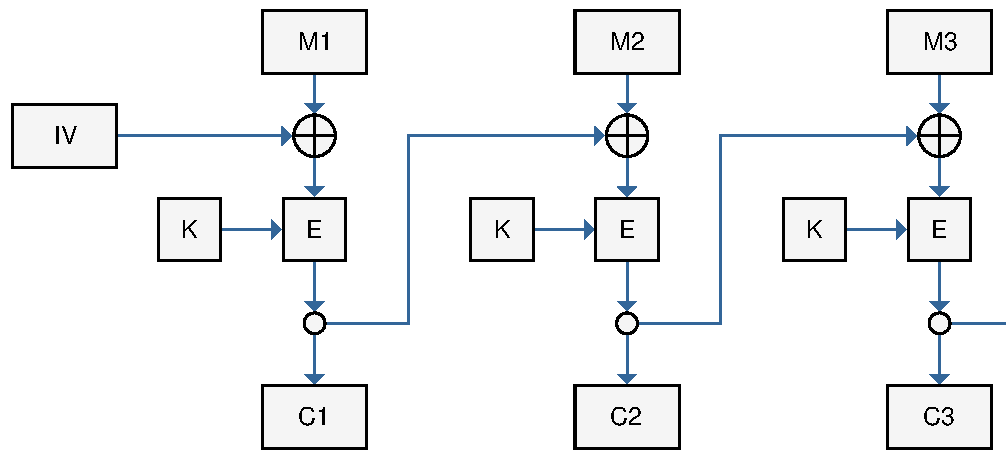
\includegraphics[width=1\textwidth]{pic/CBC}
	\caption{Режим сцепления блоков шифртекста}
	\label{fig:CBC}
\end{figure}

Благодаря сцеплению, \emph{одинаковым} блокам открытого текста соответствуют \emph{различные} шифрованные блоки. Это затрудняет криптоаналитику статистический анализ потока шифрованных блоков.

На приёмной стороне расшифрование осуществляется по правилу:
\[ \begin{array}{l}
    D_K(C_j) = M_j \oplus C_{j-1}, ~ j=1, 2, \dots, n,\\
    M_{j} = D_K(C_j) \oplus C_{j-1}.
\end{array} \]

Блок $C_0 = \textrm{IV}$ должен быть известен легальному получателю шифрованных сообщений. Обычно криптограф выбирает его случайно и вставляет на первое место в поток шифрованных блоков. Сначала передают блок $C_0$, а затем шифрованные блоки $C_1, C_2, \ldots, C_n$.

В разных пакетах блоки $C_0$ должны выбираться независимо. Если их выбрать одинаковыми, то возникают проблемы, аналогичные проблемам в режиме ECB. Например, часто первые нешифрованные блоки $M_1$ в разных пакетах бывают одинаковыми. Тогда одинаковыми будут и первые шифрованные блоки.

Однако случайный выбор векторов инициализации также имеет свои недостатки. Для выбора такого вектора необходим хороший генератор случайных чисел. Кроме того, каждый пакет удлиняется на один блок.

Для каждого сеанса передачи пакета нужны такие процедуры выбора $C_0$, которые известны криптографу и легальному пользователю. Одним из решений является использование так называемых \emph{одноразовых меток}. Каждому сеансу присваивается уникальное число. Его уникальность состоит в том, что оно используется только один раз и никогда не должно повторяться в других пакетах. В англоязычной научной литературе оно обозначается как \emph{Nonce}, то есть сокращение от <<Number used once>>\index{одноразовая метка}.

Обычно одноразовая метка состоит из номера сеанса и дополнительных данных, обеспечивающих уникальность. Например, при двустороннем обмене шифрованными сообщениями одноразовая метка может состоять из номера сеанса и индикатора направления передачи. Размер одноразовой метки должен быть равен размеру шифруемого блока. После определения одноразовой метки $\textrm{Nonce}$ вектор инициализации вычисляется в виде:
    \[ C_0 = \textrm{IV} = E_K(\textrm{Nonce}). \]

Этот вектор используется в данном сеансе для шифрования открытого текста в режиме CBC. Заметим, что блок $C_0$ передавать в сеансе необязательно, если приёмная сторона знает заранее дополнительные данные для одноразовой метки. Вместо этого достаточно вначале передать только номер сеанса в открытом виде. Принимающая сторона добавляет к нему дополнительные данные и вычисляет блок $C_0$, необходимый для расшифрования в режиме CBC. Это позволяет сократить издержки, связанные с удлинением пакета. Например, для шифра AES длина блока $C_0$ равна $16$ байтов. Если число сеансов ограничить величиной $2^{32}$ (вполне приемлемой для большинства приложений), то для передачи номера пакета понадобится только $4$ байта.

Преимущества:
\begin{itemize}
	\item отсутствие статистической зависимости блоков открытого текста и шифртекста;
\end{itemize}

Недостатки:
\begin{itemize}
	\item необходимость дополнения открытого текста до размера, кратного размеру блоку шифрования;
	\item невозможность параллельного шифрования (для следующего блока необходимо знать результат обработки предыдущего);
	\item ошибка передачи бита блока шифртекста приводит к ошибке расшифровки блока открытого текста целиком и к ошибке в одном бите следующего блока;
	\item не обеспечивает целостность.
\end{itemize}

Говоря о возможности восстановления после ошибок передачи, в режиме CBC при изменении одного бита блока шифртекста будет полностью некорректно расшифрован соответствующий блок отрытого текста, а также единственный бит \emph{следующего} блока открытого текста. Однако последующие блоки затронуты не будут. Поэтому данный режим относят к \emph{самовосстанавливающимся}.

Данный режим (как и большая часть остальных рассмотренных режимов) обеспечивает только конфиденциальность\index{конфиденциальность} передачи данных, но не целостность\index{целостность}. В модели активного злоумышленника, если последний предполагает о возможном содержимом первого блока открытого текста, а вектор инициализации передаётся в открытом виде по каналу связи, злоумышленник может подменить данные в векторе инициализации таким образом, чтобы сформировать нужное содержимое первого блока открытого текста. Такое изменение в режиме CBC не повлечёт других изменений и не приведёт к <<мусору>> в остальных блоках -- будет затронут только первый блок открытого текста. Изменение может не быть замечено получателем и привести к таким действиям получателя, которые ожидает злоумышленник, а не легальный отправитель.

\subsection{Обратная связь по выходу}
\selectlanguage{russian}

В предыдущих режимах входными блоками для функции шифрования были непосредственно блоки открытого текста. В режиме обратной связи по выходу (\langen{Output Feedback, OFB}, рис.~\ref{fig:OFB}) блоки открытого текста непосредственно на вход функции шифрования не поступают. Вместо этого функция шифрования генерирует псевдослучайный поток байтов (\emph{гамму}), который суммируется побитово по модулю $2$ с открытым текстом для получения шифртекста. Шифрование осуществляют по правилу:
\[ \begin{array}{l}
    K_0 = \textrm{IV}, \\
    K_j = E_K(K_{j-1}), ~ j = 1, 2, \dots, n, \\
    C_j = K_j \oplus M_j.
\end{array} \]

\begin{figure}[bt]
	\centering
	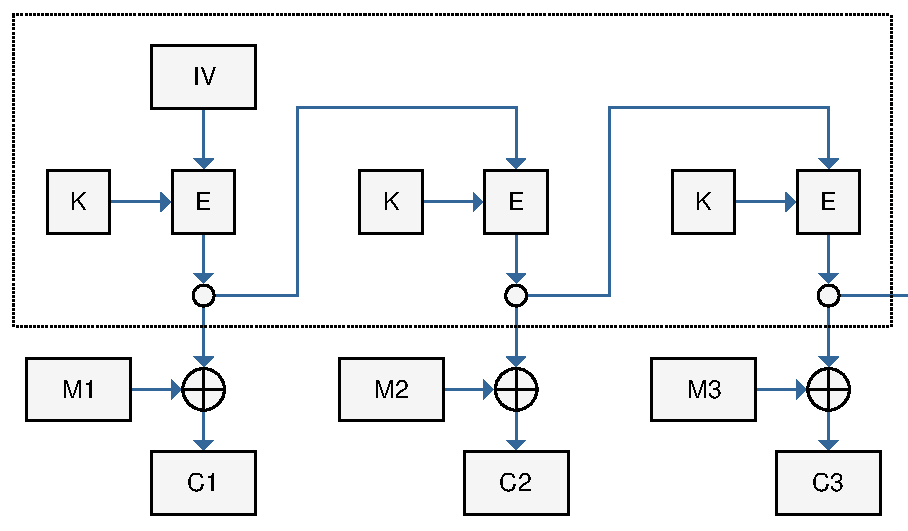
\includegraphics[width=1\textwidth]{pic/OFB}
	\caption{Режим обратной связи по выходу. Пунктирной рамкой выделена область формирования \emph{гаммы}, независящей от открытого текста.}
	\label{fig:OFB}
\end{figure}

Здесь текущий ключ $K_j$ есть результат шифрования предыдущего ключа $K_{j-1}$. Начальное значение $K_0$ известно криптографу и легальному пользователю. На приёмной стороне расшифрование выполняют по правилу:
\[ \begin{array}{l}
    K_0 = \textrm{IV}, \\
    K_j = E_K(K_{j-1}), ~ j = 1, 2, \dots, n, \\
    M_j = K_j \oplus C_j.
\end{array} \]

Как и в режиме CBC, вектор инициализации $\textrm{IV}$ может быть выбран случайно и передан вместе с шифрованным текстом, либо вычислен на основе одноразовых меток. Здесь особенно важна уникальность вектора инициализации.

Преимущества:
\begin{itemize}
	\item относительно простая реализация -- операции шифрования и расшифрования совпадают;
	\item нет необходимости дополнять открытый текст до размера, кратного размеру блоку шифрования;
	\item возможность частичной параллелизации шифрования (можно сгенерировать гамму до получения открытого текста);
	\item ошибка передачи одного бита приводит к ошибке в единственном бите открытого текста.
\end{itemize}

Недостатки:
\begin{itemize}
	\item непредсказуемый период (размер <<гаммы>>);
	\item не обеспечивает целостность.
\end{itemize}

Если рассматривать шифрование в режиме OFB как генератор псевдослучайной последовательности (<<гаммы>>), то очевидно, что максимальный период генератора равен $2^n$ блоков, где $n$ -- размер блока в битах. То есть максимальный период в битах равен $2^n \times n$. Однако нет никаких гарантий, что период будет максимален. Используя формулу из задачи о парадоксе дней рождения (см~\autoref{section:birthday-paradox}), находим, что математическое ожидание числа блоков, по достижению которого вероятность <<зациклиться>> более $1/2$, равно:

\[
b_{1/2} \geq \sqrt{2 \ln 2 \cdot N} \gtrapprox {1,18} \sqrt{N},
\]
где $N$ -- количество разных блоков. Так как $N = 2^n$, то

\[
b_{1/2} \gtrapprox \{1,18\} \sqrt{2^n} \gtrapprox {1,18} \cdot 2^{n/2}.
\]

Для шифров <<Кузнечик>> и AES $b_{1/2} \approx {1,18} \cdot 2^{64}$.

Данная оценка показывает математическое ожидание числа блоков. Но в реальности зацикливание может произойти даже на первом блоке, если в результате шифрования вектора инициализации $\textrm{IV}$ снова получится значение $\textrm{IV}$. Что фактически может привести к очень небезопасному шифрованию на гамме (<<гаммирование>>) с длиной периода всего в $n$ бит, где $n$ -- размер блока шифрования.

Хорошим размером гаммы считается такой, который больше размера шифруемого сообщения. То есть гамма не должна повторяться в рамках одной передачи. Теоретически можно ввести процесс отслеживания повтора гаммы (что на выходе функции шифрования получилось значение, равное $\textrm{IV}$) и перезапускать процесс передачи с другим значением вектора. Но это потребует усложнения режима шифрования, а также может привести к серьёзным проблемам, если при передаче нового значения $\textrm{IV}$ возникнет ошибка.

Данный режим (как и большая часть остальных рассмотренных режимов) обеспечивает только конфиденциальность\index{конфиденциальность} передачи данных, но не целостность\index{целостность}. В модели активного злоумышленника, если последний может предположить о содержимом любой части открытого текста, злоумышленник может поменять отдельные биты шифртекста, что приведёт к предсказуемым (с точки зрения криптоаналитика) изменениям в расшифрованном тексте.

\subsection{Обратная связь по шифртексту}
\selectlanguage{russian}

В режиме обратной связи по шифртексту (\langen{Cipher FeedBack, CFB}, рис.~\ref{fig:CFB}) ключ $K_j$ получается с помощью процедуры шифрования предыдущего шифрованного блока $C_{j-1}$. Может быть использован не весь блок $C_{j-1}$, а только его часть. Как и в предыдущем случае, начальное значение ключа $K_0$ известно криптографу и легальному пользователю:
\[ \begin{array}{l}
    K_0 = \textrm{IV}, \\
    K_j = E_K(C_{j-1}), ~ j = 1, 2, \dots, n,\\
    C_j = K_j \oplus M_j.
\end{array} \]

\begin{figure}[bt]
	\centering
	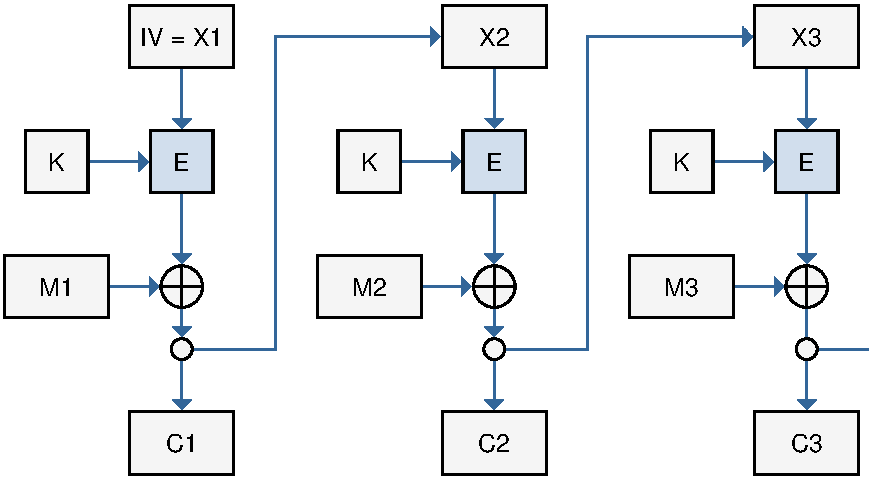
\includegraphics[width=1\textwidth]{pic/CFB}
	\caption{Режим обратной связи по шифртексту}
	\label{fig:CFB}
\end{figure}

У этого режима нет особых преимуществ по сравнению с другими режимами.


\subsection{Режим счётчика}
\selectlanguage{russian}

\begin{figure}[bt]
	\centering
	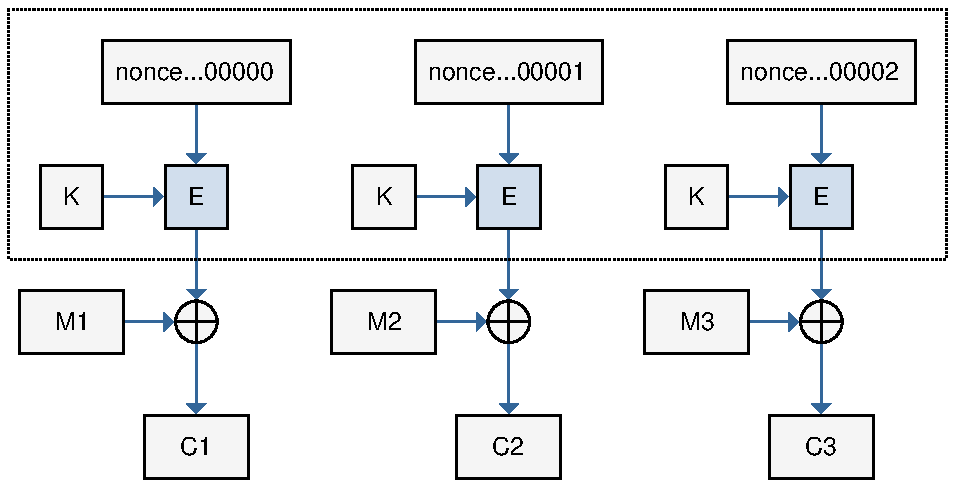
\includegraphics[width=1\textwidth]{pic/CTR}
	\caption{Режим счётчика. Пунктирной рамкой выделена область формирования \emph{гаммы}, независящей от открытого текста.}
	\label{fig:CTR}
\end{figure}

В режиме счётчика (\langen{Counter, CTR}, рис.~\ref{fig:CTR}) правило шифрования имеет вид, похожий на режим обратной связи по выходу (OFB), но позволяющий вести независимое (параллельное) шифрование и расшифрование блоков:
\[ \begin{array}{l}
    K_j = E_K(\textrm{Nonce} ~\|~ j - 1), ~ j = 1, 2, \dots, n, \\
    C_j = M_j \oplus K_j,
\end{array} \]
где $\textrm{Nonce} ~\|~ j - 1$ -- конкатенация битовой строки одноразовой метки $\textrm{Nonce}$ и номера блока, уменьшенного на единицу.
%Для стандарта AES значение $\textrm{Nonce}$ занимает 16 бит, номер блока -- 48 бит. С одним ключом выполняется шифрование $2^{48}$ блоков.

Правило расшифрования идентичное:
\[ \begin{array}{l}
    M_j = C_j \oplus K_j. \\
\end{array} \]


\subsection{Режим имитовставки}\index{имитовствка!(}
\selectlanguage{russian}

Режим выработки имитовставки (рис.~\ref{fig:GOST_MAC}, \cite{GOST-89}) принципиально отличается от рассмотренных ранее режимов тем, что призван обеспечивать не конфиденциальность, а целостность. Результатом является блок данных фиксированного размера (в ГОСТ 28147-89 -- до 32 бит), длина которого не зависит от длины исходного сообщения.

\begin{figure}[bt]
	\centering
	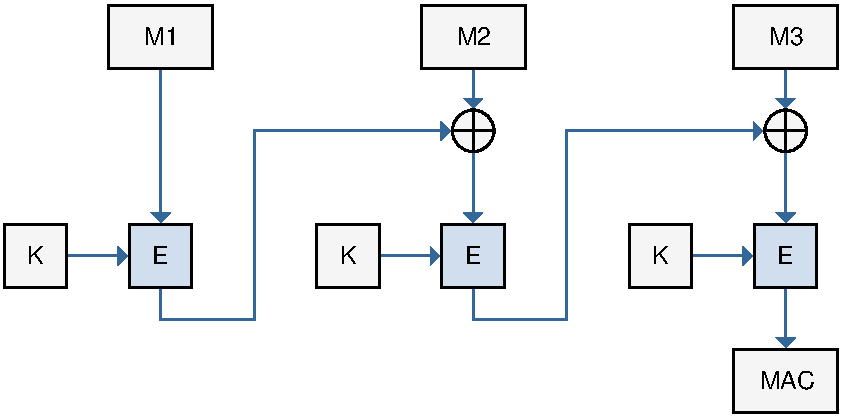
\includegraphics[width=1\textwidth]{pic/GOST_MAC}
	\caption{Режим выработки имитовставки}
	\label{fig:GOST_MAC}
\end{figure}

Входное сообщение как и ранее разбивается на блоки равной длины $M_1, M_2, \dots, M_n$. Последний блок, при необходимости, дополняется (ГОСТ 28147-89 -- нулями). Формула выработки имитовставки выглядит следующим образом:

\[ \begin{array}{l}
	X_1 = M_1; \\
	Y_j = E_K ( X_j ), ~ j = 1, 2, \dots, n; \\
	X_j = Y_{j-1} \oplus M_j, ~ j = 2, \dots, n; \\
	\textbf{MAC} = Y_n.
\end{array} \]

В ГОСТ 28147-89 для режима выработки имитовставки функция шифрования использует 16 раундов вместо 32.

Как уже было сказано, данный режим обеспечивает только целостность информации. Причём саму информацию необходимо передавать, и, возможно, шифровать отдельно. Режим не обеспечивает возможности параллельных вычислений для разных блоков открытого текста.

Принципиальным недостатком является необходимость использовать секретный ключ\index{ключ!секретный} как для выработки имитовставки, так и для её валидации (путём повторной выработки на принимающей стороне и сравнения с результатом). Позже мы рассмотрим функциональных электронных цифровых подписей, которые по своему назначению схожи с имитовставкой, но обеспечивают вариант более гибкого использования -- без необходимости раскрытия ключа, используемого для генерации ЭЦП.

\index{имитовствка!)}

\subsection{Счётчик с аутентификаций Галуа}
\selectlanguage{russian}

Режим счётчика с аутентификацией Галуа был предложен Девидом МакГрю и Джоном Виега в 2004 году (\langen{Galois/Counter Mode, GCM}, рис.~\ref{fig:GCM}, \cite{McGrew:Viega:2004}). Данный режим обеспечивает одновременно конфиденциальность и целостность, при условии правильного использования.

\begin{figure}[bt]
	\centering
	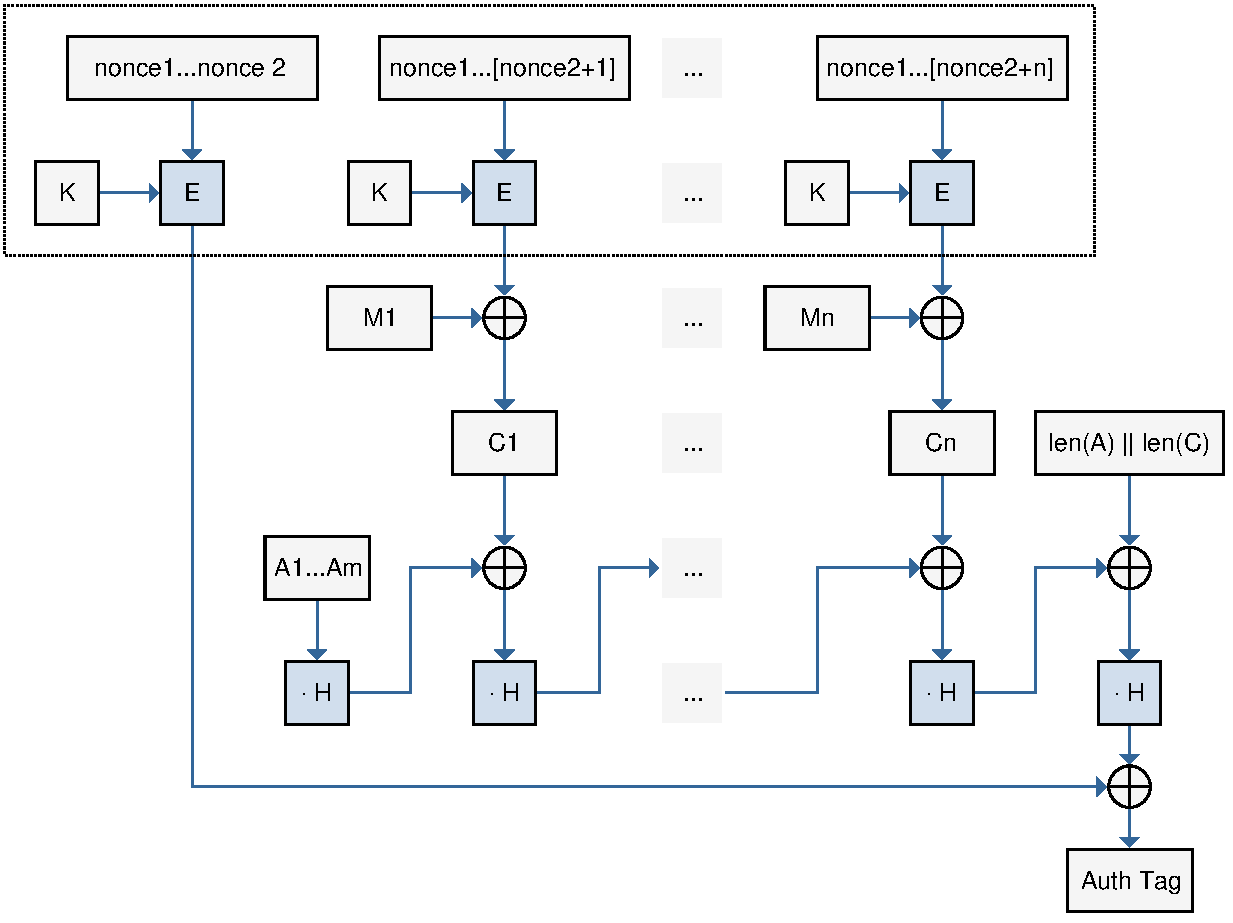
\includegraphics[width=1\textwidth]{pic/GCM}
	\caption{Режим счётчика с аутентификаций Галуа. Пунктирной рамкой выделена область формирования \emph{гаммы}, независящей от открытого текста.}
	\label{fig:GCM}
\end{figure}

Результатом работы режима, кроме набора шифроблоков, является тег аутентификации, который должен быть использован принимающей стороной для проверки целостности сообщения. Как и в режиме выработки имитовставки, генерация данного тега возможна только легальным пользователем -- знающим секретный ключ, который был использован для шифрования данных.

<<Верхняя>> часть режима является режимом работы счётчика. В качестве первого значения берётся дополнение нулями вектора инициализации до размера обрабатываемого блока. Потом, как и в режиме CTR, правая часть увеличивается на 1 для каждого следующего блока. Значения счётчика шифруются на секретном ключе $K$ для получения блоков гаммы. Самый первый блок полученной гаммы используется не для шифрования открытого текста, а для формирования тега аутентификации.

Сам тег аутентификации вырабатывается следующим образом. На вход <<подрежима>> генерации тега сначала (опционально) подаются дополнительные данные (\langen{additional authenticated data, AAD}), которые не нужно шифровать в режиме GCM, но которым нужно обеспечить целостность. Например, это может быть заголовок передаваемого пакета данных. После того, как эти данные закончатся, на вход начнут подаваться блоки шифротекста $C_1, C_2, \dots, C_n$. Использование блоков шифротекста, а не открытого текста, позволяет получателю проверить целостность передаваемых данных до того, как приступит к расшифровке. В качестве последнего блока выступает конкатенация длин дополнительных данных и открытого текста.

Формирование тега происходит через побитовое сложение результата предыдущего блока с новым блоком AAD или $C_j$ и умножение результата на константу $H$, которая в двоичном виде равна результату шифрования нулевого вектора (блока, заполненного нулями) на ключе $K$:

\[ \begin{array}{l}
	H = E_K ( 0^{\{n\}} ) \\
\end{array} \]

Умножение на константу $H$ происходит в поле Галуа $\GF{2^{n}}$. Рекомендуемый порождающий многочлен поля для шифра AES (с размером блока 128 бит):

\[ \begin{array}{l}
	f(x) = x^{128} + x^7 + x^2 + x + 1.
\end{array} \]

Результат умножения самого последнего блока побитово складывается с первым блоком сформированной гаммы.

Данный режим обеспечивает и конфиденциальность, и целостность. Шифровать отдельные блоки можно параллельно, а вычисление тега аутентификации делается намного быстрее, чем шифрование. Однако любая ошибка передачи приведёт к вычислению некорректного тега аутентификации, а отличить изменение текста в результате ошибки передачи от вмешательства злоумышленника принципиально невозможно.
